\section{Analysis of the Continuous Controller}\label{analysisController}
A first analysis of the controller can be done through the resultant Nyquist plot.

\begin{figure}[H] 
	\centering 
	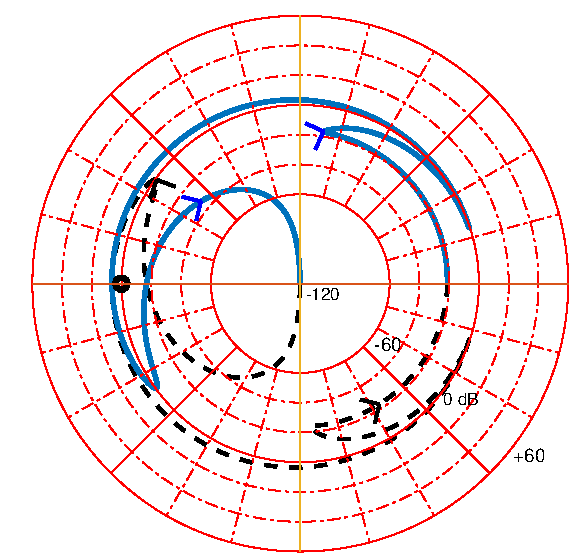
\includegraphics[scale=0.46]{figures/nyquistController}	
	\caption{Nyquist plot of the system with the controller}
	\label{nyquistController}
\end{figure}

Now the number of poles in the RHP is two and the number of encirclements around -1 is equals -2 (they are counterclockwise). This means that the system is stable, as the number of zeros in the RHP becomes 0.

Another step in the analysis is by means of a simulation, usng the block diagram of the plant.

%The resultant system can be seen in figures \figref{}.

When a reference of 0 rad is given to the system, which has a tiny deviation from the equilibrium position in the initial condition, the behavior is the one shown in \figref{TorqueResponse} and \figref{PositionResponse}.

\begin{minipage}{\linewidth}
	\begin{minipage}{0.45\linewidth}
		\begin{figure}[H]
			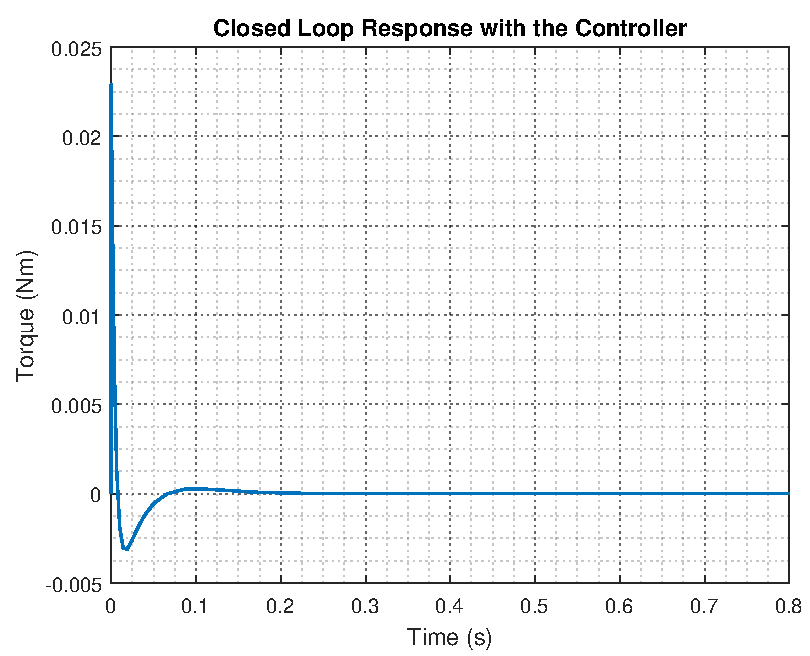
\includegraphics[scale=.56]{figures/TorqueResponse}
			\centering
			\captionsetup{justification=centering}
			\captionof{figure}{Torque needed at the motor}
			\label{TorqueResponse}
		\end{figure}
	\end{minipage}
	\hspace{0.03\linewidth}
	\begin{minipage}{0.45\linewidth}
		\begin{figure}[H]
			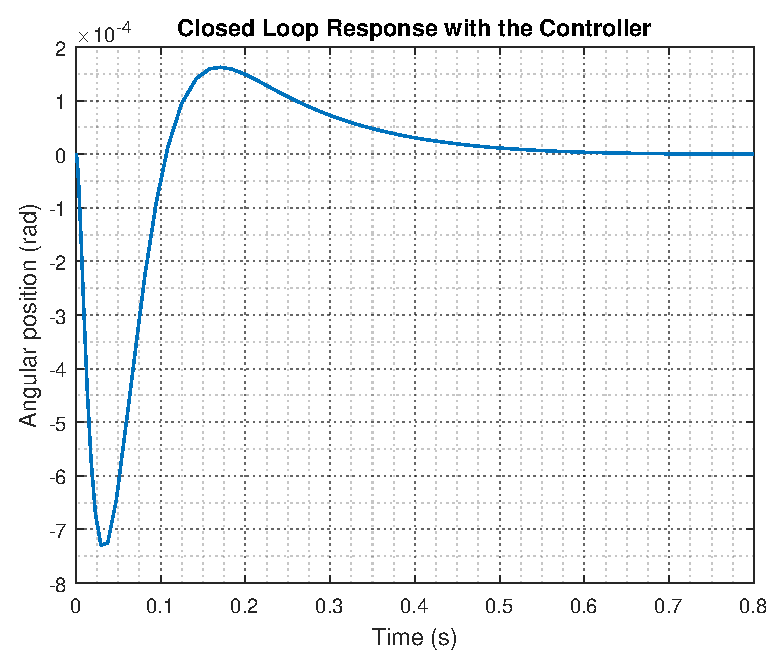
\includegraphics[scale=.56]{figures/PositionResponse}
			\centering
			\captionsetup{justification=centering}
			\captionof{figure}{Angular position of the system}
			\label{PositionResponse}
		\end{figure}
	\end{minipage}
\end{minipage}

As it can be seen, the controller is capable of balancing the Cubli at position 0 rad with a control action (torque) which can only take values from -0.134 to 0.134 as the real actuator does.